% TODO
% Clean up results
% Write temporal and graph match stuff
% Complexity analysis of new algorithm

\RequirePackage[l2tabu, orthodox]{nag}
\documentclass[envcountsame]{llncs}
\usepackage[pdftex]{graphicx}
\usepackage{booktabs}
\usepackage{microtype}
\usepackage{pgfplots}
\usepackage{pgfplotstable}
\usepackage{url}
\pgfplotsset{compat=newest}
\usepgfplotslibrary{groupplots}
\usetikzlibrary{positioning}

\pgfplotstableread{data/tanksoarcues.dat}{\tanksoardata}
\pgfplotstableread{data/2048cells.dat}{\twentyfortyeightcells}
\pgfplotstableread{data/2048eps.dat}{\twentyfortyeighteps}

\begin{document}

\title{An Episodic Memory Retrieval Algorithm for the Soar Cognitive Architecture}
\author{Francis Li, Jesse Frost, Braden J. Phillips}
\institute{School of Electrical and Electronic Engineering, University of Adelaide, SA, Australia \\
  \email{\{francis.li,jesse.frost,braden.phillips\}@adelaide.edu.au}}
\maketitle

\begin{abstract}

  Episodic memory in cognitive architectures allows intelligent agents to query their past experiences to influence decision making.
  Episodic memory in the Soar cognitive architecture must efficiently encode, store, search and reconstruct episodes as snapshots of short term working memory.
  The performance of the current search algorithm can be improved by doing a structural match phase first on all stored data and enforcing arc consistency in the first stage of the structural match.
  We demonstrate experimentally the performance of the improved search algorithm in two Soar environments.

\end{abstract}

\section{Introduction}

  \subsection{The Soar Cognitive Architecture}

  The Soar cognitive architecture is a model of cognition based on a symbolic production rule system.
  Soar models problem solving by moving an agent through the problem state-space.
  At each step it uses a decision making algorithm to decide how to modify the problem state \cite{laird12}. 
  
  Soar internally models the problem state in temporary memory called \emph{Working Memory} (WM), which consists of a set of 3-tuples called \emph{Working Memory Elements} (WMEs).
  Each WME consists of symbols which are respectively named the identifier, attribute and value.
  Together, all WMEs in WM represent a connected, directed, rooted graph where:
  \begin{itemize}
    \item identifiers represent inner nodes;
    \item attributes represent edge labels; and
    \item values represent leaf nodes or inner nodes.
  \end{itemize}
  Figure \ref{fig:wm_diagram} shows an example of how WMEs are mapped to the graph representation in Soar.
  The state of an agent's WM represents its current knowledge of the problem state.
  The agent moves through the problem state-space by adding, removing and changing WMEs.
  In this way, the graph structure represented by WM changes over time.

  \begin{figure}
  \centering
  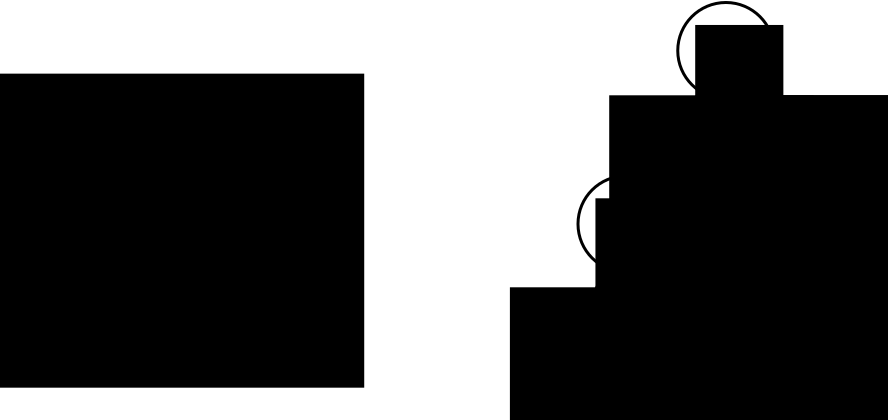
\includegraphics[scale=0.3]{graphics/wm_diagram.pdf}
  \caption{A set of WMEs on the left and the associated graph representation on the right. In this example \texttt{S1},
  \texttt{A1} and \texttt{B1} are \emph{identifiers}, \texttt{thing} and \texttt{value} are \emph{attributes}
  and \texttt{a}, \texttt{b} and \texttt{c} are \emph{values}.}
  \label{fig:wm_diagram}
  \end{figure}

  \subsection{Soar's Episodic Memory Implementation}

  In addition to WM, Soar can make use of \emph{Episodic Memory} (EpMem) to assist its decision making process.
  EpMem automatically stores the state of WM at a specified phase in each decision cycle.
  It maintains a complete history of the state of WM throughout the agent's existence as a set of snapshots of WM, where each snapshot is an \emph{episode}.

  During any cycle the agent can \emph{query} EpMem to find past experiences similar to its current state and use past decisions to influence its decision process in the present.
  It does this by providing EpMem with a cue --- a data structure representing the pattern to search for \cite{laird2008extending}.
  EpMem searches its history and returns the most recent episode containing an instance of the cue structure \cite{nuxoll2004cognitive}.
  Figure \ref{fig:epmem_diagram} illustrates the relationship between Soar's WM and EpMem.
  
  \begin{figure}
  \centering
  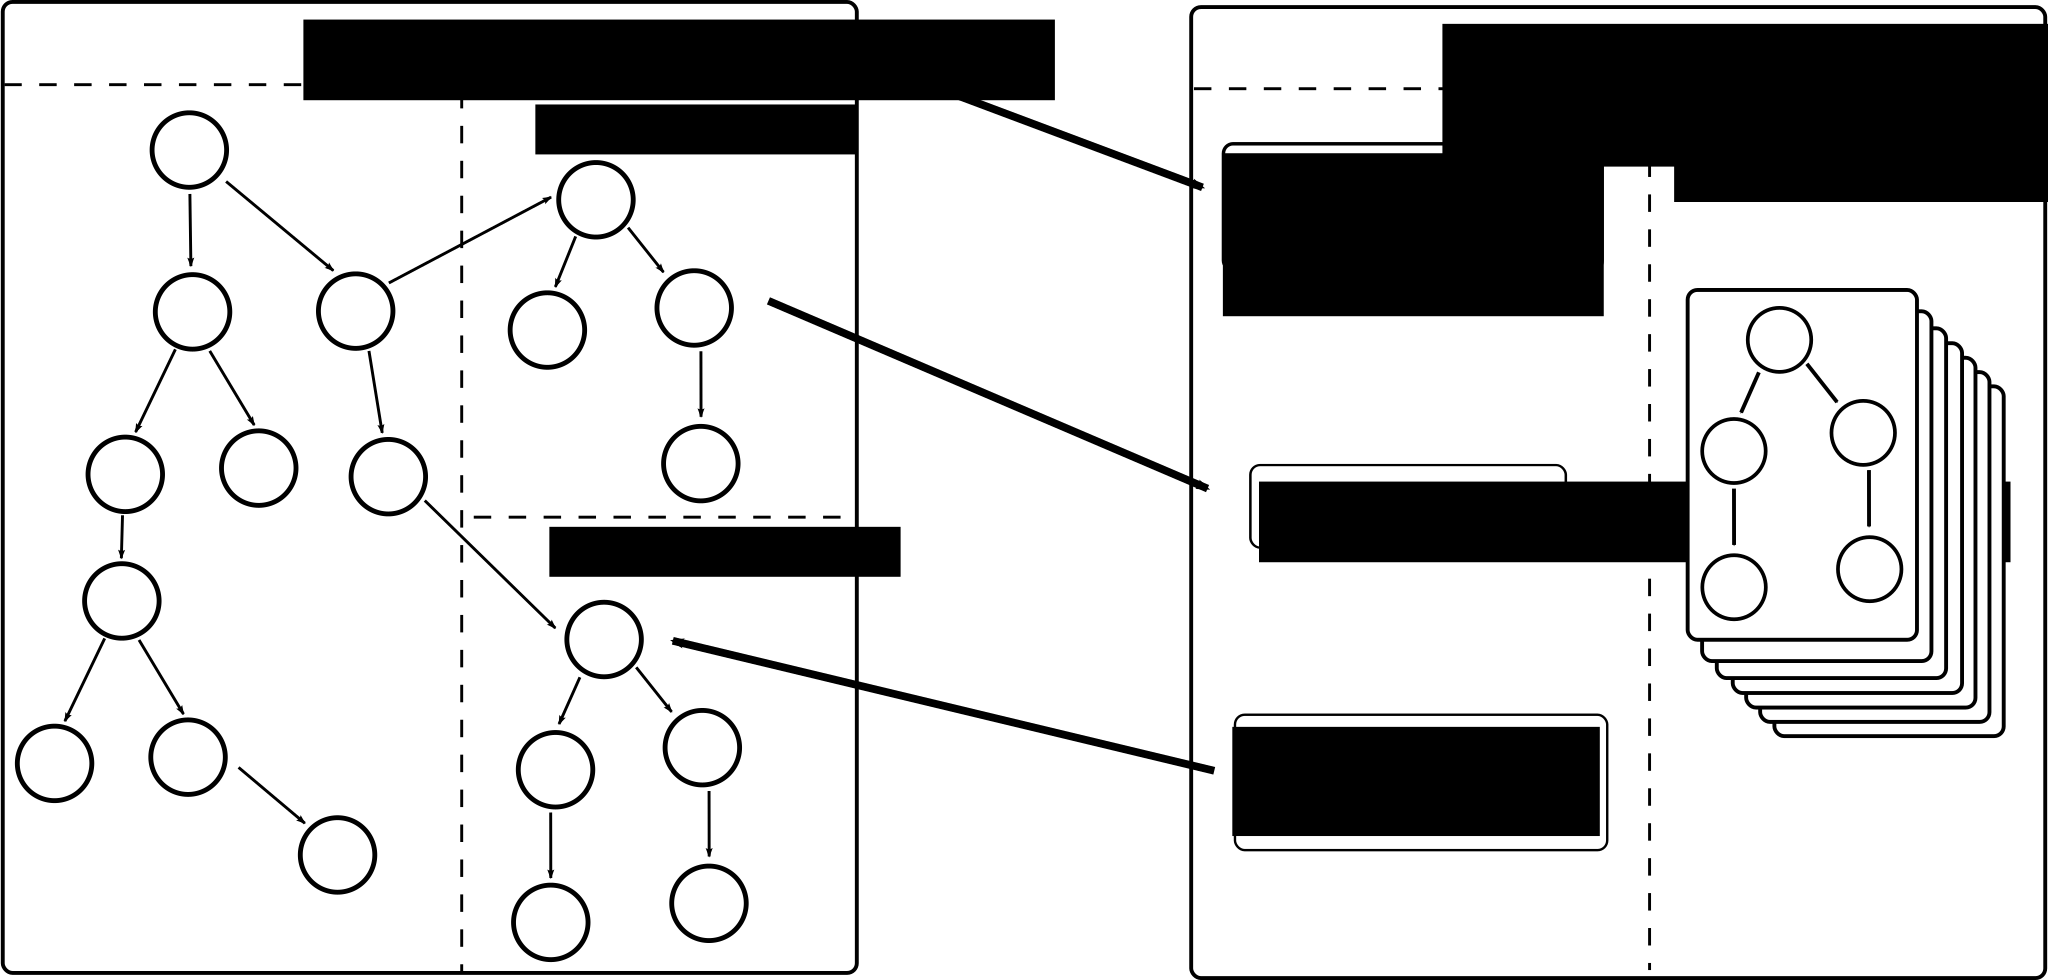
\includegraphics[scale=0.15]{graphics/epmem_diagram.pdf}
  \caption{The relationship between EpMem and WM in Soar.
  Episodes are stored in EpMem as encoded representations of WM and are retrieved by searching and matching against a cue.}
  \label{fig:epmem_diagram}
  \end{figure}

  A complete detailed description of the current implementation of EpMem in Soar can be found in
  \cite{derbinsky2012effective}.
  An EpMem implementation must be able to:
  \begin{itemize}
  \item Efficiently encode, store and index a large set of slowly changing episodes.
  \item Rapidly find the episode that best matches a cue according to some `best match' criteria.
  \item Reconstruct/decode the matching episode and return it in the agent's WM.
  \end{itemize}
  
  \subsubsection{Encoding and storage.}
  Soar's current implementation of EpMem exploits the temporal redundancy of episodes; since WM changes slowly, episodes that are close in time share many common WMEs.
  Episodes are encoded by separating structural and temporal information.
  The history of all structures that have appeared in WM is stored in the \emph{Working Memory Graph} (WMG) --- an encoding of every WME that has ever appeared in any episode\footnote{EpMem does not actually store certain working memory structures, such as those related to the EpMem interface itself.}.
  Each entry in the WMG contains an index to a table of \emph{intervals}.
  This table encodes the episodes for which each structure in the WMG was present in WM.
  The interval table is updated when a WME is added or deleted, therefore the size of the episode store increases linearly with the number of \emph{changes} to WM between episodes.
  
  \subsubsection{Cue matching.}
  \label{sec:soarcuematch}
  A cue is a set of WMEs which together represent a rooted, directed, acyclic \emph{subgraph} of WM.
  A match for a cue is defined as the most recent episode that shares the greatest number of features in common with the cue leaf nodes.
  The cue matching algorithm uses a two phase process to avoid performing a complete graph match for every stored episode:
  an episode is only a candidate for the graph match if it contains all \emph{surface} features of the cue, where a surface feature is a unique directed path from root to leaf.
  The matching algorithm searches for candidate episodes by `walking' backwards through the interval table.
  Each interval represents an episode where the state of WM changed.
  For each change, the state of satisfaction of the surface features is updated by propagating changes through a \emph{DNF graph} \cite{derbinsky2009efficiently} compiled from the cue.

  A perfect surface match does not guarantee that the cue structure was found in a past episode, only that all surface features were present.
  A structural graph match step is used to determine whether the cue structure is present within the candidate episode using a simple backtracking algorithm.
  If this search succeeds, the episode is returned, otherwise the interval walk continues.
  If the interval walk exhausts the episode store, the most recent episode with the highest surface match score is returned.

  \subsubsection{Reconstruction.}
  The reconstruction algorithm takes an episode number from the cue matching algorithm and returns the full episode to the agent in WM.
  Further details of episode reconstruction are outside the scope of this discussion.

  \subsection{Contributions}
  
  Searching EpMem is an instance of the NP-complete \emph{subgraph isomorphism} problem.
  Soar reduces the search cost by implementing a two-phase matching algorithm as described previously in section \ref{sec:soarcuematch}.
  Although this algorithm is effective, there are certain WM and cue structures for which retrievals perform poorly.
  We address these issues by making the following contributions:
  \begin{itemize}
    \item
      We describe the structural match as a constraint satisfaction problem (CSP) (Section \ref{sec:newstructural}).
      Soar's structural match has not been extensively studied \cite{derbinsky2012effective}, so formalising the search under a known framework allows us to leverage well-known techniques to improve search time cost.
      We enforce arc consistency to tighten the constraints before backtracking, thus reducing the amount of dead-ends hit during search.
    \item
      We perform the structural match before checking that the temporal information is consistent (Section \ref{sec:newstructural}, \ref{sec:temporal}). This allows us to do the most constrained search first, and ensures that the graph match is performed only once.
    \item
      We show that the proposed algorithm obtains comparable performance on most cues, and exceeds performance for cues where the original algorithm performs poorly (Section \ref{sec:results}).
  \end{itemize}
  

% TODO change section title
\section{A New Episodic Memory Retrieval Algorithm} 

  Soar's retrieval algorithm terminates quickly if a surface match is likely to correspond with a complete graph match. However:
  \begin{itemize}
    \item
      If the stored episodes contain many structures that return perfect surface matches, but fail the structural graph match, the graph match step will be executed many times.
    \item
      If the cue contains WMEs which have the same identifier and attribute but different values (multi-valued attributes), the backtracking step could reach many dead-ends and backtrack frequently.
  \end{itemize}
  
  We propose an alternative search algorithm which:
  \begin{itemize}
    \item
      Performs the structural match once before doing the interval walk; this removes the possibility of repeating the graph match and avoids the first slow retrieval scenario.
    \item
      Tightens constraints before backtracking to avoid the second slow retrieval scenario.
  \end{itemize}
  
  \subsection{Structural Match}
  \label{sec:newstructural}
  Finding an instance of the cue structure in the WMG is a constraint satisfaction problem.
  A constraint satisfaction problem (CSP) is defined as a set of variables $\mathcal{X}=\{X_1, X_2, \dots X_n\}$, a set of constraints $\mathcal{C} = \{C_1, C_2, \dots C_m\}$ and a set of non-empty domains $\mathcal{D}=\{D_1, D_2, \dots D_n\}$ \cite{dechter2003constraint}.
  
  \begin{itemize}
    \item The variable $X_i\in X$ may take on a value from $D_i\in D$.
    \item The $k$-ary constraint $C_i$ is a pair $\langle S_i, R_i\rangle$ where $S_i \subset \mathcal{X}$, called the scope of $C_i$, is a
      subset of $k$ variables $(X_{i_1}, \dots, X_{i_k})$ and
      $R_i \subset D_{i_1}\times \dots \times D_{i_k}$ is a $k$-ary relation on $S_i$.
    \item A unary constraint is one for which $k=1$ and a binary constraint is one for which $k=2$.
  \end{itemize}
  
  An instantiation of the variables is an assignment of values to each variable from the corresponding
  domain. An instantiation satisfies a constraint $C_i$ if it satisfies the relation $R_i$. An instantiation that
  satisfies all constraints is a solution to the CSP.
  
  We can define an EpMem cue to be a set of $n$ WMEs $\{W_1, \dots W_n\}$.
  For each unique inner node label in this set, define a variable $X_j$ and a domain $D_j$ which is the set of all unique inner node labels stored in the WMG.
  For each $W_i\in\{W_1, \dots W_n\}$, define a constraint $C_i$.
  If $W_i$ has a single inner node label (i.e., if it represents an edge terminating on a leaf node), $C_i$ is a unary constraint.
  If $W_i$ has two inner node labels (i.e., if it represents an edge between two inner nodes), $C_i$ is a binary constraint.
  A WME in the WMG satisfies the relation $R_i$ if the corresponding edge labels and leaf nodes match the corresponding edge labels and leaf nodes in $W_i$.

  Solutions to a CSP are generated through search.
  Simple backtracking is a depth-first search where partial instantiations are extended by assigning values to variables and then ensuring that all constraints are still satisfied.
  If a constraint is violated, the search has reached a \emph{dead-end} and must backtrack by changing the newly assigned variable's value to another in its domain.
  A depth first search is $O(b^d)$, where $b$ is the branching factor (the size of the domains) and $d$ is the depth (the number of variables).
  We can reduce the search space by preprocessing the problem to reduce the sizes of the domains.

  A CSP is \emph{arc-consistent} if any value in the domain of a variable can be extended consistently by any other variable.
  Enforcing arc consistency shrinks the domains of all variables and makes search more efficient.
  The \emph{revise} operation enforces \emph{directional arc-consistency} (DAC) between two variables $x_i$ and $x_j$ between which there is a binary constraint $C_ij$ by deleting all values in the domain $D_i$ of $x_i$ that are not in the relation $R_ij$.
  The complexity of revise is $O(b^2)$, as every value in $D_i$ must be compared with every value in $D_j$.
  However, this is reduced to $O(b)$ in practice, as domains are stored in a hashed data structure.

  A \emph{constraint graph} is a graphical representation of a CSP, where variables are nodes, and constraints are edges between nodes.
  If a constraint graph is a tree under some ordering $d = (x_1,\dots,x_n)$, then we can enforce DAC along that ordering $d$ by ensuring that every variable $x_i$ is arc-consistent relative to every variable $x_j$ such that $i \leq j$ (see \cite{dechter2003constraint}).
  This performs the revise operation at most $c$ times, where $c$ is the number of binary constraints (i.e., the number of WMEs in the cue).
  So enforcing DAC has time complexity $O(cb)$.

  The cue is rooted and acyclic and always reduces to a tree constraint graph.
  As a result, the total cost of doing the structural match is the time taken to enforce DAC added to the time needed to generate all solutions through backtracking.
  The backtracking stage is much more efficient as dead-ends are never hit.
  All generated solutions are sent to the temporal match for the next phase of processing.

  \subsection{Temporal Match}
  \label{sec:temporal}

  Solutions from the structural graph match phase must be checked to ensure that each WME was present in WM at the \emph{same} time --- that is, during a single episode.
  We compile the solutions into a data structure that tracks satisfaction of structural solutions as we walk through the intervals (in contrast to the DNF graph, which tracks satisfaction of surface features).
  This data structure is effectively a conjunctive normal form (CNF) statement, comprised of a conjunction of clauses (which are the WMEs in the cue), where each clause is a disjunction of literals (possible values which WMEs may take on).

  As we proceed with the interval walk, we keep track of the number of clauses that are `on'.
  If this count reaches the maximum possible, then a solution is present in the same episode and we can return the episode number to the EpMem reconstruction algorithm.
  If not, we proceed until the interval walk exhausts all episodes, then return the episode with the maximum count.

  The definition of a \emph{partial match} has changed from the number of surface features to the number of structural solution WMEs present. It remains to be seen how this affects agents that rely on partial match in their decision cycles. However, this temporal match algorithm can be modified to support the traditional partial match criteria by altering the compilation step.
  There is further scope for study and optimisation of the temporal match component.

  
\section{Experiments}
  \label{sec:results}

  We used two environments to evaluate EpMem algorithm performance:
  \begin{itemize}
    \item \emph{TankSoar}\footnote{\url{http://soar.eecs.umich.edu/articles/downloads/domains/176-tanksoar}} --- a computer simulation
  that uses Soar agents to control virtual tanks that navigate a two-dimensional map; we chose TankSoar because it was used in \cite{derbinsky2012effective} as a test environment to evaluate the original EpMem algorithm.
    \item A simple implementation of the popular computer game \emph{2048}\footnote{Original version available: \url{http://gabrielecirulli.github.io/2048/}}  (where a player, in this case a Soar agent, must move a set of tiles around on a four-by-four grid).
    We selected this as it produced WM structures similar to those that caused slower performance in the TankSoar environment.
  \end{itemize}

  The TankSoar agent \emph{mapping-bot} receives sensor information on its input-link, and keeps track of the game's map internally.
  The 2048 environment models its game state as a four-by-four grid. Each cell in the grid has a column, row and value.
  The 2048 agent searches for past episodes that match some number of cells (see Figure \ref{fig:tfe_cues}).
  
  We used the existing Soar EpMem search implementation and four different cues to search EpMem ranging in size from 1 to 320000 episodes generated from the TankSoar environment.
  These cues were taken from test data in \cite{derbinsky2012effective} and can be seen in Figure \ref{fig:tanksoar_cues}.
  We then performed the test on the same EpMem data using the proposed algorithm implemented in the Java programming language.

  We also used both search implementations to search for cues containing between 1 and 16 `cells' in episodic memory of up to 900 episodes generated by the 2048 environment.
  The structure of these cues is shown in Figure \ref{fig:tfe_cues}.
  
  \begin{figure}
  \centering
  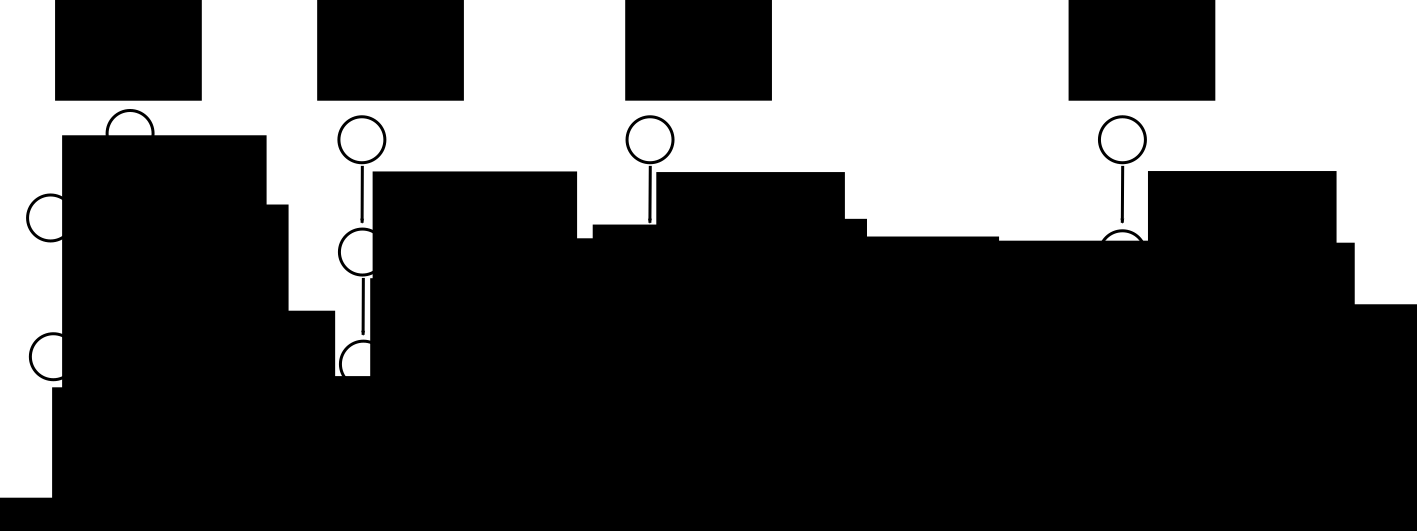
\includegraphics[scale=0.3]{graphics/tanksoar_cues.pdf}
  \caption{From left to right, cue 1, cue 2, cue 3 and cue 4 used to search TankSoar's EpMem.}
  \label{fig:tanksoar_cues}
  \end{figure}
  
  \begin{figure}
  \centering
  \includegraphics[scale=0.3]{graphics/tfe_cues.pdf}
  \caption{The cue structure used by the 2048 agent contains 1-16 `cell' structures.}
  \label{fig:tfe_cues}
  \end{figure}
  
  \subsection{Results}

 The run times for both search implementations in the TankSoar environment is shown in Figure \ref{fig:runtime_comparison1}.
 Both were comparable in performance, with the proposed algorithm having a small advantage despite the addition of the preprocessing step.
  % move 10^5 to axis title
  % Change one line to dotted
  % Move legend
  \begin{figure}
    \begin{tikzpicture}
      \begin{groupplot}[
        group style={
            group name=tanksoar cues,
            group size=2 by 2,
            xlabels at=all,
            ylabels at=all,
            horizontal sep=1.5cm,
            vertical sep=2.3cm
        },
        width=6cm,
        xlabel=\# of episodes (10\textsuperscript{5}),
        ylabel=time $t$ (ms),
        legend entries={Current, New},
        legend style={at={(0.5,1.02)},anchor=south},
        legend columns=2,
        xtick scale label code/.code={}
      ]
        \nextgroupplot
          \addplot table [x={numeps}, y={cue8soar}] {\tanksoardata};
          \addplot table [x={numeps}, y={cue8new}] {\tanksoardata};
        \nextgroupplot
          \addplot table [x={numeps}, y={cue12soar}] {\tanksoardata};
          \addplot table [x={numeps}, y={cue12new}] {\tanksoardata};
        \nextgroupplot
          \addplot table [x={numeps}, y={cue13soar}] {\tanksoardata};
          \addplot table [x={numeps}, y={cue13new}] {\tanksoardata};
        \nextgroupplot
          \addplot table [x={numeps}, y={cue15soar}] {\tanksoardata};
          \addplot table [x={numeps}, y={cue15new}] {\tanksoardata};
      \end{groupplot}
      \node[above = .7cm of tanksoar cues c1r1.north] {Cue 1};
      \node[above = .7cm of tanksoar cues c2r1.north] {Cue 2};
      \node[above = .7cm of tanksoar cues c1r2.north] {Cue 3};
      \node[above = .7cm of tanksoar cues c2r2.north] {Cue 4};
    \end{tikzpicture}
    \caption{The search time for the four TankSoar cues. Both algorithms are comparable except for cue 2, where the new algorithm is an order of magnitude better.}
    \label{fig:runtime_comparison1}
  \end{figure}
 Figure \ref{fig:cellograph} shows the run time for a search in the 2048 episodic memory using both
  algorithms with cues containing between 1 and 4 cells.
  The proposed algorithm was consistently able to reduce the variable domains to a single element, which resulted in backtrack-free structural match.
  The original Soar implementation consistently passed the surface match phase and triggered a graph match for many intervals.
  The unreduced domains caused near worst case time for each repeated attempt at structural graph match.
  We attempted to test cues with more than 4 cells, but tests required too much time to execute (greater than 30 minutes).

  Figure \ref{fig:episodograph} shows the search times for a cue consisting of two cells and an episodic memory of 1 to 900 episodes.
  The original Soar implementation was in some cases able to complete the search early when the graph match phase matched early in the interval walk, but in other cases ended up attempting an expensive graph match many times.
  The proposed algorithm  consistently performed better as it performed the graph match only once in each search and was able to reduce each domain to a single element each time.

  \begin{figure}
    \begin{tikzpicture}
    \begin{axis}[
      xlabel=\# of cells,
      ylabel=time $t$ (10\textsuperscript{4} ms),
      width=7.3cm,
      legend entries={Current, New},
      legend style={at={(.02, .98)}, anchor=north west},
      xtick={0,...,4},
      ytick scale label code/.code={},
      name=tfecell
    ]
      \addplot table [x={numcells}, y={soartime}] {\twentyfortyeightcells};
      \addplot table [x={numcells}, y={newtime}] {\twentyfortyeightcells};
    \end{axis}
    \node [right=of tfecell] {
    \pgfplotstabletypeset[
      columns/numcells/.style={column name=Cells},
      columns/soartime/.style={column name=Current},
      columns/newtime/.style={column name=New},
      every head row/.style={
      before row={%
      \toprule
      & \multicolumn{2}{c}{Time (ms)}\\},after row=\midrule},
      every last row/.style={
      after row=\bottomrule},
]\twentyfortyeightcells};
    \end{tikzpicture}
    \caption{Average search time for Soar increases exponentially as the number of cell structures in the cue are increased.}
	\label{fig:cellograph}
  \end{figure}

  \begin{figure}
    \begin{tikzpicture}
    \begin{axis}[
      xlabel=\# of episodes,
      ylabel=time $t$ (ms),
      legend entries={Current, New},
      width=7.3cm,
    ]
      \addplot table [x={numeps}, y={soartime}] {\twentyfortyeighteps};
      \addplot table [x={numeps}, y={newtime}] {\twentyfortyeighteps};
    \end{axis}
    \node [right=of tfecell] {
    \pgfplotstabletypeset[
      columns/numeps/.style={column name=Episodes},
      columns/soartime/.style={column name=Current},
      columns/newtime/.style={column name=New},
      every head row/.style={
      before row={%
      \toprule
      & \multicolumn{2}{c}{Time (ms)}\\},after row=\midrule},
      every last row/.style={
      after row=\bottomrule},
]\twentyfortyeighteps};
    \end{tikzpicture}
    \caption{Average search time for Soar vs. current implementation with 2-cell cue. Soar's performance is highly dependent on the number of times it needs to do a graph match.}
	\label{fig:episodograph}
  \end{figure}
   
\section{Conclusion}
  
  Soar's EpMem system has an effective encoding and cue matching algorithm.
  However, certain episode and cue structures can significantly reduce its performance by causing repeated attempts at performing a full graph match, or by stressing the simple backtracking algorithm.

  We have proposed an alternative cue matching system that performs an efficient graph match first before attempting the interval search.
  The graph match enforces arc consistency before backtracking to tighten the constraints and avoid dead-ends.
  An implementation of this approach in the Java programming language provides comparable performance to the current algorithm in most cases, and significant improvements in situations where: (a) there are frequently perfect surface matches, yet the structural graph match fails;
  or (b) the structural graph match hits many dead-ends and backtracks frequently.

  In addition, the proposed algorithm can extend EpMem to handle cyclic and non-rooted cues and has scope for further optimisation.

\bibliographystyle{splncs03}
\bibliography{epmem}
\end{document}